%%%%%%%%%%%%%%%%%%%%%%%%%%  example_doublecolumn.tex  %%%%%%%%%%%%%%%%%%%%%%%%%%%%%%%%
%
% This is example_twocolumn.tex, an example file for use with the SIAM LaTeX2E
% Proceedings macros. It is designed to provide two-column output. Please take
% the time to read the following comments, as they document how to use the
% SIAM Proceedings macro files. This file can be composed and printed out for
% use as sample output.
%
% Please submit suggestions for changes to: tex@siam.org.
%
% This file is to be used as an example for style only. It should not be read
% for content.

%%%%%%%%%%%%%%% PLEASE NOTE THE FOLLOWING STYLE RESTRICTIONS %%%%%%%%%%%%%%%

%%  1. There are no new tags.  Existing LaTeX tags have been formatted to match
%%     the SIAM Proceedings style.
%%
%%  2. Do not change the margins or page size!  Do not change from the default
%%     text font or the default text size of 10pt!
%%
%%  3. We recommend that you use BibTeX and siamplain.bst to list your references.
%%     You can use \cite in the text to mark your reference citations and
%%     \bibitem in the listing of references at the end of your chapter. See
%%     the examples in the following file. If you do use BibTeX, please supply
%%     your bib or bbl file with the manuscript file.
%%
%%  4. This macro is set up for two levels of headings (\section and
%%     \subsection). The macro will automatically number the headings for you.
%%
%%  5. No running heads are to be used.
%%
%%  6. Theorems, Lemmas, Definitions, Equations, etc. are to be double numbered,
%%     indicating the section and the occurrence of that element within that 
%%     section. (For example, the first theorem in the second section would be 
%%     numbered 2.1. The macro will automatically do the numbering for you.
%%
%%  7. Figures and Tables must be single-numbered. Use existing LaTeX tags for 
%%     these elements. Numbering will be done automatically.
%%
%%  8. Page numbering is not included in this macro since pagination
%%     will be set by the program committee.
%%

\documentclass[twoside,leqno,twocolumn]{article}

% Comment out the line below if using A4 paper size
\usepackage[letterpaper]{geometry}

\usepackage{siamproceedings}

\usepackage[T1]{fontenc}
\usepackage{amsfonts}
\usepackage{graphicx}
\usepackage{epstopdf}
\usepackage{enumitem}
\usepackage{algorithmic}
\ifpdf
  \DeclareGraphicsExtensions{.eps,.pdf,.png,.jpg}
\else
  \DeclareGraphicsExtensions{.eps}
\fi

% Add a serial/Oxford comma by default.
\newcommand{\creflastconjunction}{, and~}

% Used for creating new theorem and remark environments
\newsiamremark{remark}{Remark}
\newsiamremark{hypothesis}{Hypothesis}
\crefname{hypothesis}{Hypothesis}{Hypotheses}
\newsiamthm{claim}{Claim}

%%Currently, the algorithm title font matches the figure and table title
%%fonts. To make the algorithm title font appear as small caps, uncomment
%%the following code:

%\makeatletter
%\renewcommand{\ALG@name}{\sc Algorithm}
%\makeatother

\usepackage{amsopn}
\DeclareMathOperator{\diag}{diag}


\begin{document}

%
\newcommand\relatedversion{}
\renewcommand\relatedversion{\thanks{The full version of the paper can be accessed at \protect\url{https://arxiv.org/abs/0000.00000}}} % Replace URL with link to full paper or comment out this line

\title{\Large SIAM/ACM Proceedings Macros for Use With LaTeX\relatedversion}
    \author{James E. Haines\thanks{Society for Industrial and Applied Mathematics (\email{jhaines@siam.org}, \email{rginder@siam.org}, \url{http://www.siam.org}).}
    \and Rachel Ginder\footnotemark[2]    
    \and Mitch C. Donovan\thanks{Department of Applied Mathematics, Fictional University, Austin, TX and NASA, Johnson Space Center, Houston, TX
  (\email{donovan@fictional.edu}, \email{mcd@nasa.gov}, \url{https://www.nasa.gov/johnson/}).}}

\date{}

\maketitle

% Copyright Statement
% When submitting your final paper to a SIAM proceedings, it is requested that you include
% the appropriate copyright in the footer of the paper.  The copyright added should be
% consistent with the copyright selected on the copyright form submitted with the paper.
% Please note that "20XX" should be changed to the year of the meeting.

% Default Copyright Statement
\fancyfoot[R]{\scriptsize{Copyright \textcopyright\ 20XX by SIAM\\
Unauthorized reproduction of this article is prohibited}}

% Depending on which copyright you agree to when you sign the copyright form, the copyright
% can be changed to one of the following after commenting out the default copyright statement
% above.

%\fancyfoot[R]{\scriptsize{Copyright \textcopyright\ 20XX\\
%Copyright for this paper is retained by authors}}

%\fancyfoot[R]{\scriptsize{Copyright \textcopyright\ 20XX\\
%Copyright retained by principal author's organization}}

%\pagenumbering{arabic}
%\setcounter{page}{1}%Leave this line commented out.

\begin{abstract} The abstract must be able to stand alone and so cannot contain citations to the paper's references, equations, etc.  An abstract must consist of a single paragraph and be concise. Because of online formatting, abstracts must appear as plain as possible. Any equations should be inline.
\end{abstract}

\section{Introduction.}
The introduction introduces the context and summarizes the manuscript. It is important to clearly state the contributions of this piece of work.

\section{Cross references and hyperlinks.}
\label{sec:cr+hyp}

The SIAM Proceedings macros support cross references and hyperlinks via the
\texttt{cleveref} and \texttt{hyperef} packages, which are loaded by default.

\subsection{Cleveref.}
\label{sec:cleveref}

SIAM strongly recommends using the commands provided by 
the \texttt{cleveref} package for cross referencing.
The package is automatically loaded and already customized
to adhere to SIAM's style guidelines. 
To create a cross reference, use the command $\backslash$\texttt{cref} (inside
sentence) or $\backslash$\texttt{Cref} (beginning of a sentence) in place of the
object name and $\backslash$\texttt{ref}. 
The \texttt{cleveref} package enhances \LaTeX's cross-referencing features, 
allowing the format of cross references to be determined automatically
according to the ``type" of cross reference (equation, section, etc.)
and the context in which the cross reference is used.
So, the package \emph{automatically} inserts the object name as well as the
appropriate hyperlink.
Additional examples are shown in the following sections for equations, 
tables, figures, sections, etc.

\subsection{Hyperef.}
\label{sec:hyperef}

Hyperlinks are created with the $\backslash$\texttt{href} and $\backslash$\texttt{url} commands.
The $\backslash$\texttt{email} command is also defined, as shown in the
Page 1 footnote below.

\section{Math and equations.}
\label{sec:math}
Here we show some example equations, with numbering, and examples of
referencing the equations. The SIAM Proceedings macro includes the package 
\texttt{amsmath} by default, and we include some of its features as
well, although the reader should consult the package user manual for
further guidance \cite{amsmath,shortmath}.
Note that several of the example are adapted from Mittlebach and Goossen's 
guide to \LaTeX~\cite{MiGo04}.

Here is a straightforward example of inline mathematics
equations that does not use any special packages or features: 
Let $S=[s_{ij}]$ ($1\leq i,j\leq n$) be a $(0,1,-1)$-matrix of order $n$.

Next we show the \texttt{smallmatrix} environment for an
inline matrix from the \texttt{amsmath} package, which is included by
default.

Matrices of no more than two rows appearing in text can be created
as shown:
$B = \bigl[ \begin{smallmatrix} B_{11} & B_{12} \\ 
  B_{21} & B_{22} \end{smallmatrix} \bigr]$.

Bigger matrices can be rendered with environments from
the \texttt{amsmath} package, such as \texttt{bmatrix} and
\texttt{pmatrix}:
\begin{equation}\label{eq:matrices}
  S=\begin{bmatrix}1&0\\0&0\end{bmatrix}
  \quad\text{and}\quad
  C=\begin{pmatrix}1&1&0\\1&1&0\\0&0&0\end{pmatrix}.
\end{equation}
\Cref{eq:matrices} above shows some example matrices.

The following shows how to use the \texttt{align} environment from
\texttt{amsmath} to easily align multiple equations.

\Cref{eq:a,eq:b,eq:c} show three aligned equations.
\begin{align} 
  f &= g, \label{eq:a} \\
  f' &= g', \quad\text{and} \label{eq:b} \\
  \mathcal{L}f &= \mathcal{L}g \label{eq:c}.
\end{align}

Another way to number a set of equations is the
\texttt{subequations} environment from \texttt{amsmath}.

We calculate the Fr\'{e}chet derivative of $F$ as follows:
\vspace{-12pt}
\begin{subequations}
\begin{align}
  F'(U,V)(H,K) = &\langle R(U,V),H\Sigma V^{T} \label{eq:aa}\\
  &+ U\Sigma K^{T} - P(H\Sigma V^{T}  \nonumber \\
  &+ U\Sigma K^{T})\rangle  \nonumber \\
  = &\langle R(U,V),H\Sigma V^{T} + U\Sigma K^{T}\rangle \nonumber \\
  = &\langle R(U,V)V\Sigma^{T},H\rangle \label{eq:bb}\\
  &+ \langle \Sigma^{T}U^{T}R(U,V),K^{T}\rangle.  \nonumber
\end{align}
\end{subequations}
We can link to \Cref{eq:aa} at the beginning of the equation and \cref{eq:bb} later in the equation separately.

For an equation split over multiple lines, the next equation shows the
usage of the \texttt{multline} environment provided by \texttt{amsmath}.

We claim that the projection $g(U,V)$ is given by the pair of matrices:
\begin{multline} \label{eq:ml}
  g(U,V) = \biggl( \frac{R(U)V\Sigma^{T}U^{T} 
    - U\Sigma V^{T}R(U)^{T}}{2}U,\\
  \frac{R(U)^{T}U\Sigma V^{T}-V \Sigma^{T}U^{T}R(U)}{2}V \biggr).
\end{multline}

\section{Theorem-like environments.}
\label{sec:thm}
The SIAM Proceedings macro loads the \texttt{ntheorem} package and uses it to define the following
theorem-like environments:
\texttt{theorem}, 
\texttt{lemma}, 
\texttt{corollary},
\texttt{definition}, and
\texttt{proposition}.
SIAM also defines a \texttt{proof} environment that automatically
inserts the symbol ``$\,\proofbox\,$'' at the end of any proof, even if it ends in an
equation environment. \emph{Note that the document may need to be
  compiled twice for the mark to appear.}
Some of the calculus examples were adapted from \cite{CalcI}. 
%
% Example theorem and lemma declarations are shown.  These
% are all numbered in the same sequence and produce labels in small caps
% with an italic body. Use the command \code{\textup} to produce Roman
% type for numbers and parentheses.
%
The following shows usage of the \texttt{theorem} environment. 
Here we state our main result as \cref{thm:bigthm}.

\begin{theorem}[$LDL^T$ Factorization \cite{GoVa13}]\label{thm:bigthm}
  If $A \in \mathbb{R}^{n \times n}$ is symmetric and the principal
  submatrix $A(1:k,1:k)$ is nonsingular for $k=1:n-1$, then there
  exists a unit lower triangular matrix $L$ and a diagonal matrix
  \begin{displaymath}
    D = \diag(d_1,\dots,d_n)
  \end{displaymath}
  such that $A=LDL^T$. The factorization is unique.
\end{theorem}

Followed by a theorem without an optional argument used to name the theorem.

\begin{theorem}\label{thm:mvt}
  Suppose $f$ is a function that is continuous on the closed interval
  $[a,b]$ and differentiable on the open interval $(a,b)$.
  Then there exists a number $c$ such that $a < c < b$ and
  \begin{displaymath}
    f'(c) = \frac{f(b)-f(a)}{b-a}.
  \end{displaymath}
  In other words,
  \begin{displaymath}
    f(b)-f(a) = f'(c)(b-a).
  \end{displaymath}
\end{theorem}

Observe that \cref{thm:bigthm,thm:mvt,cor:a} correctly mix references
to multiple labels.

\begin{corollary}\label{cor:a}
  Let $f(x)$ be continuous and differentiable everywhere. If $f(x)$
  has at least two roots, then $f'(x)$ must have at least one root.
\end{corollary}
\begin{proof}
  Let $a$ and $b$ be two distinct roots of $f$.
  By \cref{thm:mvt}, there exists a number $c$ such that
  \begin{displaymath}
    f'(c) = \frac{f(b)-f(a)}{b-a} = \frac{0-0}{b-a} = 0.
  \end{displaymath}
\end{proof}
Note that we can also alter the proof environment.
\begin{proof}[Proof of \cref{thm:mvt}]
We now show...
\end{proof}

The macro also defines commands to create your own theorem- and
remark-like environments:
\begin{itemize}[nosep]
\item \texttt{newsiamthm} --- Small caps header, italized body. 
\item \texttt{newsiamremark} --- Italics header, roman body.
\end{itemize}
Each command takes two arguments. The first is the environment name,
and the second is the name to show in the document. These commands should
be used instead of $\backslash$\texttt{newtheorem}.

NOTE: Due to a current limitation of \texttt{cleveref}, any custom defined theorem-like environment 
aside from the ones listed in the SIAM Style Manual \cite[Chapter 6]{siam} will need to use $\backslash$\texttt{ref} 
instead of $\backslash$\texttt{cref} when referenced in the document.  The theorem-like
environments listed in the style manual that are safe to use with \texttt{cleveref} are 
\texttt{theorem}, 
\texttt{lemma}, 
\texttt{corollary},
\texttt{definition},
\texttt{proposition},
\texttt{fact}, 
\texttt{claim}, 
\texttt{conclusion},
\texttt{result}, 
\texttt{consequence}, and
\texttt{problem}.

An additional note is that 
\texttt{fact}, 
\texttt{claim}, 
\texttt{conclusion},
\texttt{result}, 
\texttt{consequence}, and
\texttt{problem} 
can also be defined as a remark-like environment in accordance with the SIAM Style Manual \cite[Chapter 6]{siam} without having 
an issue with \texttt{cleveref} if an author chooses to do so.

%\vspace{-12pt}
\section{Figures.}
\label{sec:fig}
It is recommended that all figures be generated in a vector format (e.g., EPS or PDF).  
If figures in a JPG or PNG format are used, make sure they are of a sufficiently high resolution. 
Make sure that your figures are optimized!  For instance, EPS and PDF figures should not have 
thousands of layers that vastly increase the file size for no benefit to image legibility.

The following is an example for how to generate \cref{fig:testfig}.  This
example uses the \texttt{graphicx} package for the
$\backslash$\texttt{includegraphics} command.

\begin{figure}[h!]
  \centering
  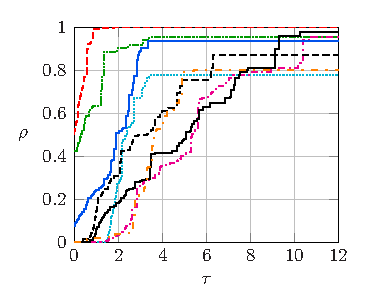
\includegraphics[width=0.65\columnwidth]{example_fig1}
  \caption{Example figure using an external image file.}
  \label{fig:testfig}
\end{figure}

If working with EPS images and using \texttt{pdflatex}, we
use the package \texttt{epstopdf} to automatically convert EPS
images to PDF for inclusion in PDF documents created by 
\texttt{pdflatex}.  Please note that \texttt{epstopdf} requires 
\texttt{texlive-font-utils} which may not be part of a standard \LaTeX\ installation.

\begin{figure*}[t!]
  \centering
  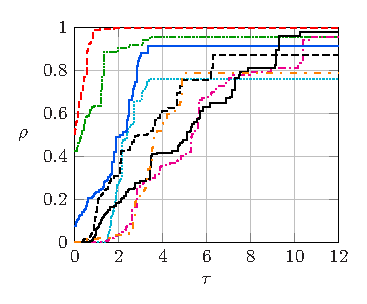
\includegraphics[width=1.5\columnwidth]{example_fig2}
  \caption{Example figure using an external image file that spans both columns.}
  \label{fig:testfig2}
\end{figure*}

\section{Tables.}
\label{sec:tab}
Table captions should go above the tables.
The following shows the code to generate \cref{tab:simpletable}.
More complicated tables can be created using subfloats via the 
\texttt{subfig} package, as well as special column options from the 
\texttt{array} package.
%\vspace{-12pt}
\begin{table}[tbhp]
\footnotesize
  \caption{Example table}\label{tab:simpletable}
\begin{center}
  \begin{tabular}{|c|c|c|} \hline
   Species & \bf Mean & \bf Std.~Dev. \\ \hline
    1 & 3.4 & 1.2 \\
    2 & 5.4 & 0.6 \\ 
    3 & 7.4 & 2.4 \\ 
    4 & 9.4 & 1.8 \\ \hline
  \end{tabular}
\end{center}
\end{table}

\section{Algorithm.}
\label{sec:alg}

The \texttt{algorithm} package is automatically included in the SIAM Proceedings
macro. This provides the float environment. Users have the choice of \texttt{algpseudocode},
\texttt{algorithmic}, and other packages for actually formatting the algorithm.
For example, \cref{alg:buildtree} is produced as follows.

\begin{algorithm}
\caption{Build tree}
\label{alg:buildtree}
\begin{algorithmic}
\STATE{Define $P:=T:=\{ \{1\},\ldots,\{d\}$\}}
\WHILE{$\#P > 1$}
\STATE{Choose $C^\prime\in\mathcal{C}_p(P) \in C^\prime := \operatorname{argmin}_{C\in\mathcal{C}_p(P)} \varrho(C)$}
\STATE{Find an optimal partition tree $T_{C^\prime}$ }
\STATE{Update $P := (P{\setminus} C^\prime) \cup \{ \bigcup_{t\in C^\prime} t \}$}
\STATE{Update $T := T \cup \{ \bigcup_{t\in\tau} t : \tau\in T_{C^\prime}{\setminus} \mathcal{L}(T_{C^\prime})\}$}
\ENDWHILE
\RETURN $T$
\end{algorithmic}
\end{algorithm}

\section{Sections.}
\label{sec:sec}
Sections are denoted using standard \LaTeX\ section commands, i.e.,
$\backslash$\texttt{section}, $\backslash$\texttt{subsection}, etc. Section heading names should end with a period to separate them from the content that follows.

Any numbered, labeled sections can be referenced using $\backslash$\texttt{cref},
including those without a title.

\subsection{Lower level sections.}
Note that there may be some variation between different proceedings regarding the use of lower level sections. 
While this SIAM Proceedings macro does support the use of $\backslash$\texttt{subsubsection}, $\backslash$\texttt{paragraph}, 
and $\backslash$\texttt{subparagraph}, authors should follow the guidelines for a given proceedings on what is and is not
allowed.

\paragraph{Paragraph.}
Here is an example of a $\backslash$\texttt{paragraph}. Paragraph and subparagraph headings are italic and not numbered.

\subparagraph{Subparagraph.}
Here is an example of a $\backslash$\texttt{subparagraph}.

\subsubsection{Subsubsection.}
Here is an example of a $\backslash$\texttt{subsubsection}.

\section{SIAM style considerations.}
\label{sec:style}
When not specifically mentioned in the given guidelines for a specific proceedings, SIAM proceedings articles should follow
SIAM's editorial style manual \cite{siam}. For instance, the serial/Oxford comma is set up in \texttt{cleveref} by default
and expected to be used throughout the article. Fonts should not be changed from the default and neither should the text size
of 10pt (with the exception being footnotesize, of course).

\subsection{Parenthetical citations.}
In accordance with SIAM's editorial style manual \cite{siam}, citations are allowed to be either parenthetical or not. For 
example, both ``Note that several of the example are adapted from Mittlebach and Goossen's guide to \LaTeX~\cite{MiGo04}." 
and ``Note that several of the example are adapted from \cite{MiGo04}." are both acceptable and such constructions are common.

\subsection{Additional requested examples.}
An example of an en-dash in a number range, e.g., 1--9.

Since mentioning it is so common, use $\backslash$\texttt{CC} to put a nicely formatted \CC~in your document.

An example of $\backslash$\texttt{textrm} within an equation to get non-math typesetting of some English words. 
$$x=y-z \quad \textrm{ for all } x.$$

Also note that $\backslash$\texttt{operatorname} can be used to define a function like $\operatorname{min}$, $\operatorname{max}$, 
$\operatorname{argmin}$, etc. (see \cref{alg:buildtree}) so that it is formatted as roman text no matter where it appears.

\section{Conclusion.}
A conclusion or summary is numbered like any other section.

\appendix
\section{An example appendix.} 
Appendices are created with the normal sectioning commands, following
the command $\backslash$\texttt{appendix}. 

\begin{lemma}
Test Lemma.
\end{lemma}

\section{An appendix regarding the Bibliography.}
\label{sec:bib}
The SIAM BibTeX style file (called \texttt{siamplain.bst}), in addition to the
standard key fields, includes the keys listed below:
\begin{itemize}[nosep]
\item \texttt{doi}: Digital object identifier, a unique alphanumeric string
\item \texttt{url}: Web address, usually impermanent
\item \texttt{urldate}: Date that the web address was last accessed
\item \texttt{eprint}: Archive identifier, a unique alphanumeric string
\item \texttt{eprintclass}: Archive class
\item \texttt{archive}: Archive URL, defaults to \nolinkurl{https://arXiv.org/abs}
\item \texttt{archivepreprint}: Archive name, defaults to ``arXiv''
\item \texttt{eid}: Article ID, if there are no page numbers
\item \texttt{pagetotal}: Total number of pages, for use with article ID
\end{itemize}
Every entry type includes an optional link to a DOI, a URL, and/or an archive 
preprint reference. Further, the \texttt{article} entry supports an Article ID, 
\texttt{eid}, and number of pages, \texttt{pagetotal}.

\subsection{Additional bibliography examples.}
Here we provide additional examples for technical reports from Cornell~\cite{Chew1989} and the University of Zurich~\cite{instance1290}
as well as a conference paper from the Proceedings of the Seventeenth Annual ACM-SIAM Symposium on Discrete Algorithms
(SODA) \cite{Aggarwal06}.

\section*{Acknowledgments.}
The acknowledgments section comes
immediately before the references and after any appendices. It should
be declared by $\backslash$\texttt{section*\{Acknowledgments\}} so that it is not numbered.

We would like to acknowledge the assistance of volunteers in putting
together these updated SIAM Proceedings macros and example files.

% SIAM recommends using BibTeX
% if using BibTeX
\bibliographystyle{siamplain}
\bibliography{example_references}
\end{document}

% else
%\begin{thebibliography}{10}
%
%\bibitem{Aggarwal06}
%{\sc G.~Aggarwal and J.~D. Hartline}, {\em Knapsack auctions}, in Proceedings
%  of the Seventeenth Annual ACM-SIAM Symposium on Discrete Algorithms (SODA),
%  Philadelphia, 2006, SIAM, pp.~1083--1092,
%  \url{http://dl.acm.org/citation.cfm?id=1109557.1109677}.
%
%\bibitem{amsmath}
%{\sc {American Mathematical Society}}, {\em User's guide for the
%  \texttt{amsmath} package (version 2.0)}, 2002,
%  \url{ftp://ftp.ams.org/pub/tex/doc/amsmath/amsldoc.pdf} (accessed
%  2015-07-30).
%
%\bibitem{Chew1989}
%{\sc L.~P. Chew}, {\em Guaranteed-quality triangular meshes}, Technical Report
%  89-983, Department of Computer Science, Cornell University, Apr. 1989.
%\newblock \url{https://hdl.handle.net/1813/6899}.
%
%\bibitem{CalcI}
%{\sc P.~Dawkins}, {\em Paul's online math notes: Calculus {I} --- notes},
%  \url{http://tutorial.math.lamar.edu/Classes/CalcI/MeanValueTheorem.aspx}
%  (accessed 2015-07-08).
%
%\bibitem{shortmath}
%{\sc M.~Downes}, {\em Short math guide for {\LaTeX}}, 2002,
%  \url{ftp://ftp.ams.org/pub/tex/doc/amsmath/short-math-guide.pdf} (accessed
%  2015-07-30).
%
%\bibitem{GoVa13}
%{\sc G.~H. Golub and C.~F. Van~Loan}, {\em Matrix Computations}, The Johns
%  Hopkins University Press, Baltimore, 4th~ed., 2013.
%
%\bibitem{MiGo04}
%{\sc F.~Mittlebach and M.~Goossens}, {\em The \LaTeX\ Companion},
%  Addison-Wesley, 2nd~ed., 2004.
%
%\bibitem{instance1290}
%{\sc B.~Stiller, T.~Bocek, F.~Hecht, G.~Machado, P.~Racz, and M.~Waldburger},
%  {\em Mobile systems {IV}}, tech. report, University of Zurich, Department of
%  Informatics, Jan. 2010.
%
%\bibitem{siam}
%{\em {SIAM} style manual: For journals and books}, 2013,
%  \url{https://epubs.siam.org/pb-assets/files/SIAM_STYLE_GUIDE_2019-1635349464967.pdf}.
%
%\end{thebibliography}
%
%\end{document}
